\section{Divide and Conquer}

%%%%%%%%%%%%%%%%%%%%
\begin{frame}{Integer multiplication (Problem 2.15)}
  \begin{exampleblock}{Integer Multiplication}
    Multiplying two $n$-bit integers in $o(n^2)$ time. {\small (Assuming $n = 2^k$.)}
  \end{exampleblock}

  \vspace{0.50cm}

  \centerline{Column multiplication in $\Theta(n^2)$}

  \begin{block}{Elementray operations:}
	\begin{itemize}
	  \item $n$-bit + $n$-bit: $O(n)$
	  \item $1$-bit $\times$ $1$-bit: $O(1)$
	  \item $n$-bit shifted by $1$-bit: $O(1)$
	\end{itemize}
  \end{block}
\end{frame}
%%%%%%%%%%%%%%%%%%%%
\begin{frame}{Integer multiplication (Problem 2.15)}
  \begin{block}{Simple divide and conquer:}
	\begin{align*}
	  x & = x_L : x_R = 2^{n/2} x_L + x_R  \\
	  y & = y_L : y_R = 2^{n/2} y_L + y_R
	\end{align*}

	\begin{align*}
	  xy & = (2^{n/2} x_L + x_R) (2^{n/2} y_L + y_R) \\
		 & = 2^{n} x_L y_L + 2^{n/2} (x_L y_R + x_R y_L) + x_R y_R
	\end{align*}

	\[
	  T(n) = 4T(n/2) + \Theta(n) = \Theta(n^2)
	\]
  \end{block}
\end{frame}
%%%%%%%%%%%%%%%%%%%%
\begin{frame}{Integer multiplication (Problem 2.15)}
  \begin{block}{A little history:}
  \begin{itemize}
    \item Kolmogorov (1952) conjecture: $\Omega(n^2)$
    \item Kolmogorov (1960) seminar
    \item Karatsuba (\emph{within a week}): $\Theta(n^{1.59})$
    \item ``The Complexity of Computations'' by Karatsuba, 1995
  \end{itemize}
  \end{block}
\end{frame}
%%%%%%%%%%%%%%%%%%%%
\begin{frame}{Integer multiplication (Problem 2.15)}
  \begin{block}{Karatsuba algorithm:}
    \[
      T(n) = 3T(n/2) + \Theta(n) = \Theta(n^{\log_{2}{3}}) = \Theta(n^{1.59})
    \]

	\pause

	\[
      xy = 2^{n} x_L y_L + 2^{n/2} (x_L y_R + x_R y_L) + x_R y_R
	\]
	
    \[
      \underbrace{(x_L + x_R) (y_L + y_R)}_{P_0} = \underbrace{x_L y_L}_{P_1} +
      (x_L y_R + x_R y_L) + \underbrace{x_R y_R}_{P_2}
    \]

    \[
      xy = 2^{n} P_1 + 2^{n/2} (P_0 - P_1 - P_2) + P_2
    \]
  \end{block}
\end{frame}
%%%%%%%%%%%%%%%%%%%%
\begin{frame}{Matrix multiplication (Problem 2.16)}
  \begin{exampleblock}{Matrix multiplication}
    Multiplying two $n \times n$ matrices in $o(n^3)$ time. {\small (Assuming $n = 2^k$.)}
    \[ Z = X \times Y \]
  \end{exampleblock}

  \vspace{0.50cm}
  \begin{columns}
    \column{0.40\textwidth}
	  \[ Z_{ij} \]

	  \[ T(n) = \Theta(n^2 \cdot n) = \Theta(n^3) \]
    \column{0.60\textwidth}
	  \begin{block}{Elementrary operations:}
	    \begin{itemize}
	      \item integer addition: $O(1)$
	      \item integer multiplication: $O(1)$
	    \end{itemize}
	  \end{block}
  \end{columns}
\end{frame}
%%%%%%%%%%%%%%%%%%%%
\begin{frame}{Matrix multiplication (Problem 2.16)}
  \begin{displaymath}
	X = \begin{bmatrix} A & B \\ C & D \end{bmatrix}, \quad
	Y = \begin{bmatrix} E & F \\ G & H \end{bmatrix} \qquad (A \ldots H \in
	\mathbb{R}^{n/2} \times \mathbb{R}^{n/2})
  \end{displaymath}

  \[
    XY = \begin{bmatrix} AE + BG & AF + BH \\ CE + DG & CF + DH \end{bmatrix}
  \]

  \[
    T(n) = 8T(n/2) + \Theta(n^2) = \Theta(n^3)
  \]
\end{frame}
%%%%%%%%%%%%%%%%%%%%
\begin{frame}{Matrix multiplication (Problem 2.16)}
  \begin{block}{Strassen algorithm:}
    \[
      T(n) = 7T(n/2) + \Theta(n^2) = \Theta(n^{\lg {7}}) = \Theta(n^{2.808})
    \]
  \end{block}

  \[
	XY = \begin{bmatrix} P_5 + P_4 - P_2 + P_6 & P_1 + P_2 \\ P_3 + P_4 & P_1 + P_5 - P_3 - P_7 \end{bmatrix}
  \]

  \begin{columns}
	\column{0.40\textwidth}
	{\footnotesize
	  \begin{align*}
		P_1 &= A(F - H) \\
		P_2 &= (A + B)H \\
		P_3 &= (C + D)E \\
		P_4 &= D(G - E) \\
		P_5 &= (A + D)(E + H) \\
		P_6 &= (B - D)(G + H) \\
		P_7 &= (A - C)(E + F)
	  \end{align*}
	}
	\column{0.60\textwidth}
	  \pause
	  \begin{itemize}
		\item Strassen (1969): $\Theta(n^{2.808})$ \\
		  ``Gaussian Elimination is Not Optimal''
		  \pause
		\item (2014): $\Theta(n^{2.373})$
		  \pause
		\item Known lower bound: $\Omega(n^{2})$
	  \end{itemize}
  \end{columns}
\end{frame}
%%%%%%%%%%%%%%%%%%%%
\begin{frame}{1-D DP}
  \begin{exampleblock}{Maximal sum subarray (Problem 1.3.5)}
    \begin{itemize}
      \item array $A[1 \cdots n], a_{i} >=< 0$
      \item to find (the sum of) an MS in $A$
    \end{itemize}
	
    \[
      A[-2,1 ,-3,4,-1,2,1,-5,4] \Rightarrow [4,-1,2,1]
    \]
  \end{exampleblock}

  \pause
  \begin{alertblock}{Trial and error.}
    \begin{itemize}
      \item try subproblem $\text{MSS}[i]$: the sum of the MS (\text{MS}[i]) in $A[1 \cdots i]$
      \item goal: $\text{mss} = \text{MSS}[n]$
      \item question: Is $a_{i} \in \text{MS}[i]$?
      \item recurrence: 
	\[ 
	  \text{MSS}[i] = \max \set{\text{MSS}[i-1], \textcolor{red}{???}}
	\]
    \end{itemize}
  \end{alertblock}
\end{frame}
%%%%%%%%%%%%%%%%%%%%
\begin{frame}{1-D DP}
  \begin{block}{Solution.}
    \begin{itemize}
      \item subproblem $\text{MSS}[i]$: the sum of the MS \textcolor{red}{\it ending with} $a_{i}$ or 0
      \item goal: $\text{mss} = \max_{1 \le i \le n} \text{MSS}[i]$
      \item<2-> question: where does the $\text{MS}[i]$ start?
      \item<2-> recurrence: 
		\[ 
		  \text{MSS}[i] = \max \set{\text{MSS}[i-1] + a_{i}, 0} \text{ \textcolor{red}{(prove it!)}}
		\]
      \item<3-> initialization: $\text{MSS}[0] = 0$
    \end{itemize}

    % \begin{displaymath}
    %   \text{MSS}[i] = \left\{ \begin{array}{ll}
    %     0 & i = 0 \\
    %     \max \set{\text{MSS}[i-1] + a_{i}, 0} & i > 0
    %   \end{array} \right.
    % \end{displaymath}
  \end{block}
\end{frame}
%%%%%%%%%%%%%%%%%%%%
\begin{frame}[fragile]{1-D DP}
  \begin{block}{Code.}
    \begin{verbatim}
      MSS[0] = 0
      For i = 1 to n
        MSS[i] = max{MSS[i-1] + A[i], 0}
      return max_{i = 1 to n} MSS[i]
    \end{verbatim}
  \end{block}

  \pause

  \begin{block}{Simpler code.}
    \begin{verbatim}
      mss = 0
      MSS = 0
      For i = 1 to n
        MSS = max{MSS + A[i], 0}
        mss = max{mss, MSS}
      return mss
    \end{verbatim}
  \end{block}
\end{frame}
%%%%%%%%%%%%%%%%%%%%
\begin{frame}{Pancake sorting (Problem 1.3.1)}
  \fignocaption{width = 0.25\textwidth}{figs/pancake-sorting.png}

  \pause
  \centerline{How to bring the biggest pancake to the bottom?}

  \pause
  \[
	T(n) = 2n-3
  \]

  \pause
  \begin{alertblock}{Reference}
	\begin{itemize}
	  \item $T(n) \le \frac{5n+5}{3}$, 1979: ``Sorting by Perfix Reversals'' \pause by Bill Gates \emph{et al.}
		\pause
	  \item $T(n) \le \frac{18n}{11}$, 2009
	\end{itemize}
  \end{alertblock}
\end{frame}
%%%%%%%%%%%%%%%%%%%%
\begin{frame}{\# Big V's (Problem 1.3.8)}
  \centerline{How many Big V's are there at most?}

  \pause
  \vspace{0.50cm}
  \centerline{``Does A follow B?''}

  \pause
  \vspace{0.50cm}
  \centerline{Don't forget to check it!}
\end{frame}
%%%%%%%%%%%%%%%%%%%%
\begin{frame}{Bolts and nuts (Problem 2.10)}
  \fignocaption{width = 0.30\textwidth}{figs/bolts-nuts.jpg}

  \pause
  \centerline{Using quicksort}

  \pause
  \[
	A(n) = O(n \log n)
  \]

  \pause
  \begin{alertblock}{Reference}
	$\Theta(n \log n)$ in the worst case:
	\begin{itemize}
	  \item ``Matching Nuts and Bolts'' by Alon \emph{et al.}, $\Theta(n \log^4 n)$
	  \item ``Matching Nuts and Bolts Optimality'' by Bradford, 1995
	\end{itemize}
  \end{alertblock}

\end{frame}
%%%%%%%%%%%%%%%%%%%%
\begin{frame}{Bolts and nuts (Problem 2.10)}
  \fignocaption{width = 0.30\textwidth}{figs/bolts-nuts.jpg}

  \[
	\Omega(n \log n)
  \]

  \pause
  \centerline{At least as hard as the sorting problem.}

  \pause
  \[
	3^{H} \ge L \textcolor{red}{\ge n!} \Rightarrow H \ge \log (n!) \Rightarrow H = \Omega(n \log n)
  \]
\end{frame}
%%%%%%%%%%%%%%%%%%%%
\begin{frame}{$K$-sorted (Problem 2.9)}
  \[
	1,\;2,\;4,\;3;\quad 7,\;6,\;8,\;5;\quad 10,\;11,\;9,\;12;\quad 15,\;13,\;16,\;14
  \]

  \pause
  \vspace{0.20cm}

  \begin{center}
	$1\text{-sorted}$? \\ \pause
	$2\text{-sorted}$? \\ \pause
	$n\text{-sorted}$?
  \end{center}

  \pause
  \[
	1\text{-sorted} \to 2\text{-sorted} \to 4\text{-sorted} \to \cdots \to n\text{-sorted}
  \]

  \pause
  \centerline{Quicksort stops after the $\log k$ recursions.}

  \pause
  \[
	O(n \log k)
  \]
\end{frame}
%%%%%%%%%%%%%%%%%%%%
\begin{frame}{$K$-sorted (Problem 2.9)}
  \[
    \Omega(n \log k)
  \]

  \pause
  \[
	L = \frac{n!}{\left( (\frac{n}{k})! \right)^{k}}
  \]

  \pause
  \[
	H \ge \log \left(\frac{n!}{\left( (\frac{n}{k})! \right)^{k}} \right)
  \]
\end{frame}
%%%%%%%%%%%%%%%%%%%%
\begin{frame}{Dutch national flag problem (Problem 2.4)}
  \begin{columns}
	\column{0.50\textwidth}
	  \fignocaption{width = 0.50\textwidth}{figs/dutch-flag.png}{\centerline{The Dutch national flag}}
	\column{0.50\textwidth}
	  \fignocaption{width = 0.35\textwidth}{figs/dijkstra.jpg}{\centerline{Edsger W. Dijkstra}}
  \end{columns}

  \vspace{0.50cm}
  \centerline{Red balls \emph{before} White balls \emph{before} Blue balls}

  \pause
  \[
	\textsc{Color}(i) \quad \textsc{Swap}(i,j)
  \]
\end{frame}
%%%%%%%%%%%%%%%%%%%%
\begin{frame}{Dutch national flag problem (Problem 2.4)}
  Loop invariant:

  \pause
  \[
    r = 0; \; w = 0; \; b = n\;
  \]

  \vspace{0.30cm}
  \begin{description}
	\item[Red:] \uncover<3->{$\textsc{Swap}(r,w); \; r = r + 1; \; w = w + 1;$}
	\item[White:] \uncover<4->{$w = w + 1;$}
	\item[Blue:] \uncover<5->{$\textsc{Swap}(b-1, w); \; b = b - 1;$}
  \end{description}
\end{frame}
%%%%%%%%%%%%%%%%%%%%
\begin{frame}{Repeated elements (Problem 2.12)}
  \begin{itemize}
	\item $R[1 \dots n]$
	\item $\text{check}(R[i], R[j])$
	\item $\# > \frac{n}{13}$
  \end{itemize}

  \pause
  \vspace{0.30cm}

  \[
	\# > \frac{n}{k}
  \]

  \begin{center}
    an $O(n \log k)$ algorithm \\
    the lower bound $\Omega(n \log k)$
  \end{center}

  \begin{alertblock}{Reference}
	``Finding Repeated Elements'' by Misra \& Gries, 1982
  \end{alertblock}
\end{frame}
%%%%%%%%%%%%%%%%%%%%
% \begin{frame}{VLSI layout}
%   \begin{exampleblock}{Problem (Area-Efficient VLSI Layout)}
%     Embedding a complete binary tree with $n$ leaves into a grid with minimum
%     area.
%     \begin{itemize}
%       \item VLSI: Very Large Scale Integration
%       \item complete binary tree circuit of $\#layer = 3,5,7,\ldots$
% %       \item $n$ leaves (\textcolor{red}{why only leaves?})
%       \item vertex on grid; no crossing edges
%       \item area = width $\times$ height
%     \end{itemize}
%   \end{exampleblock}
% \end{frame}
% %%%%%%%%%%%%%%%%%%%%
% \begin{frame}{VLSI layout}
%   Na\"{\i}ve embedding:
%    \[ H(n) = H(\frac{n}{2}) + \Theta(1) = \Theta(\lg n) \]
%    \[ W(n) = 2W(\frac{n}{2}) + \Theta(1) = \Theta(n) \]
%    \[ A(n) = \Theta(n \lg n) \]
% \end{frame}
% %%%%%%%%%%%%%%%%%%%%
% \begin{frame}{VLSI layout}
%   Smart (H-Layout) embedding:
%   \[ \Box \times \Box = n? \; 1 \times n;\; \frac{n}{\lg n} \times \lg n;\;
%   \textcolor{blue}{\sqrt{n} \times \sqrt{n}}
%   \]
%   Goal: $H(n) = \Theta(\sqrt{n}); W(n) = \Theta(\sqrt{n}); A(n) = \Theta(n).$
%   \pause
%   \[
% 	H(n) = \Box H(\frac{n}{\Box}) + O(\Box); H(n) = 2 H(\frac{n}{4}) +
% 	O(n^{\frac{1}{2} - \epsilon})
%   \]
%   \pause
%   \[ H(n) = 2H(\frac{n}{4}) + \Theta(1) \]
%   \pause
%   \centering \textcolor{blue}{Here it is: H-Layout}
% \end{frame}
% %%%%%%%%%%%%%%%%%%%%
% \begin{frame}{VLSI layout}
%   \begin{figure}[htp]
% 	\begin{center}
% 	  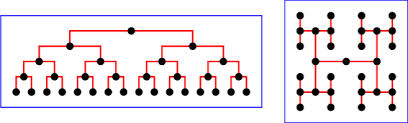
\includegraphics[width = 0.80\textwidth]{figs/vlsi}
% 	\end{center}
%   \end{figure}
% \end{frame}
%%%%%%%%%%%%%%%%%%%%
\begin{frame}[noframenumbering]
  \fignocaption{width = 0.50\textwidth}{figs/thankyou.jpg}
\end{frame}
%%%%%%%%%%%%%%%%%%%%
% \begin{frame}{Counting inversions (Problem 2.11)}
% \end{frame}
%%%%%%%%%%%%%%%%%%%%
% \begin{frame}{Maxima-finding (Problem 2.14)}
%   \centerline{Wrong recursions!}
%   \pause
%   \vspace{0.30cm}
% 
%   \centerline{3D?}
%   \pause
%   \vspace{0.30cm}
% 
%   \centerline{Lower bound $\Omega(n \log n)$!}
% \end{frame}
%%%%%%%%%%%%%%%%%%%%
